\begin{figure}[t]
  \centering
  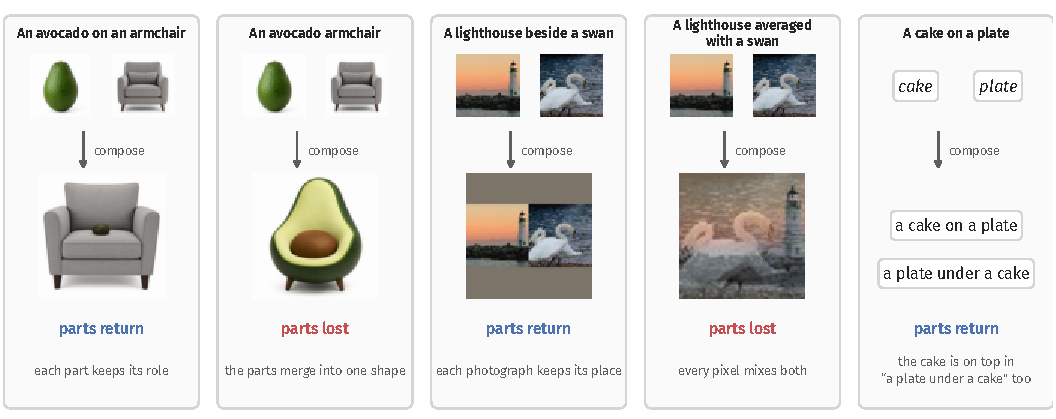
\includegraphics[width=\linewidth]{fig_intro.pdf}
  \caption{\textbf{Some wholes give their parts back, and others blend them.} Each column composes two parts into a whole. Placing an avocado on an armchair, setting two photographs side by side and naming two nouns in a sentence keep each part in its role, so the whole comes apart again (blue). An avocado-shaped armchair and the pixel average of two photographs merge the parts, and many pairs of parts give the same whole (red). Canva's text-to-image tool generated the avocado and armchair images \citep[after][]{openai2021dalle}, and the photographs come from Tiny-ImageNet \citep{le2015tiny}.}
  \label{fig:intro}
\end{figure}
